
\section{实验环境与评价指标}

因为我们找不到任何拓扑带有SRLG链路属性,所以我们通过注入SRLG信息生成一个合成的数据集。拓扑数据有$\TopoNum$种不同的拓扑,具有不同的节点数目、链路数目、链路权重(表示链路的延迟或其他参数),如表\ref{tab:AllSample}所示显示了拓扑的基本属性。这7个拓扑中的节点、链路)。

\begin{table*}[htbp]
\caption{SRLG拓扑数据}
  \centering
\footnotesize{  \begin{tabular}{*{18}{c}}
\toprule
拓扑 & 1 & 2 & 3 & 4 & 5 & 6& 7   \\
\midrule
点   &     527&      521    &      521     &    2023             &     451     &     521     &     449       \\
边   &    4158 &  4052     &    4152      &   4142          &       2780   &      4052   &      2778    \\
%Graph density  & 1.5\% &    1.49\% &   1.52\%  &  0.1\%  &   0.10\% &   1.41\%  &  1.5\% &   1.38\%   \\
No.SRLG & 132 &  86   &  89  &  207        & 210  &  128  &   88    \\
SRLG边比率 & 9.66\% & 6.16\% &   6.18\% &   14.94\%    &   22.55\%  &  9.65\% &   9.53\%     \\
\bottomrule
\end{tabular}
}
\label{tab:AllSample}
\end{table*}

为了进行性能比较,除了我们的算法(名为\CI),我们还实现了另外四个SRLG不相交路径对算法。算法如下:
\begin{enumerate}
  \item ILP:\cite{hu2003diverse} 中的工作旨在寻找SRLG不相交路径对。通过整数线性规划方程使这两条路径总的权重最小化。我们没有找到其他通过整数线性规划方程寻找Min-Min SRLG不相交路径对的方法的研究。因此,从\cite{hu2003diverse}的整数规划方程,通过改变目标函数构造Min-Min SRLG 不相交路径对问题的整数线性规划方程。
  \item IQCP:因为任意0−-1整数线性规划方程,其中所有变量为0或1,原问题的整数线性规划方程可以表示为一个二次约束方程,我们还设计了Min-Min SRLG 不相交路径问题成一个整数二次约束规划(IQCP)\cite{hu2003diverse}。
  \item KSP\cite{eppstein1998finding}:它在源节点$s$和目的节点$d$中找到第K短路作为候选AP路径,一个接一个地测试候选的AP路径是否有相应的SRLG不相交路径BP,直到我们发现了这样的BP,算法才结束。
  \item CoSE\cite{rostami2007cose}:当AP遇到陷阱问题时,CoSE尝试进行简单而详尽的搜索,以找到一个SRLG集合。任何AP路径通过这个SRLG集都无法找到SRLG不相交的BP路径。基于这个SRLG集合,它划分原问题并设计算法来求SRLG不相交路径对。
\end{enumerate}


前两者(ILP和IQCP)是基于整数规划模型的。在我们的实现中,工具GUROBI 7.0\cite{optimization2012gurobi}用于解决这两个整数规划问题。六种性能指标用于评估不同的SRLG分路径算法:
\begin{itemize}
  \item 路径权重:路径中链路权重的总和。
  \item 路径跳数:路径中的跳数。
  \item 运行时间:查找SRLG不相交路径对的归一化平均时间。
  \item 算法加速比:给定两种不同的算法($alg_1$ 和$alg_2$)的计算时间,表示为$T_1$ 和 $T_2$,算法$alg_1$对于算法$alg_2$计算时间上的加速比是$alg_1$: ${S_{1 - 2}} = T_1/T_2$。
  \item 核加速比:并行程序的核心加速比\cite{grama2003introduction}通常定义为$S_P=\frac{T_1}{T_p}$,其中p是处理器内核和$T_1$和$T_p$表示在1核和$p$核上的运行时间。
  \item 效率\cite{grama2003introduction}:定义为$E_p=\frac{S_p}{p}=\frac{T_1}{pT_p}$,它是百分比(0,1)的范围内。


\end{itemize}


所有实现都是在linux服务器上运行的,这个服务器配置Intel(R) Xeon(R) CPU E5-2620  2.00GHz(24 核)和32.00GB内存。为了测量计算时间,我们在所有实现的算法中插入一个定时器。

我们通过在拓扑数据集里注入SRLG链路属性产生了两种SRLG类型,星型类型和非星型类型。在光纤网络中,SRLG是星型类型,而在其他网络类型中,例如一个Overlay网络中,SRLG可以是非星型的。每个SRLG组是通过随机选择2-5链路组成的。在五种SRLG不相交路径对算法中,只有CoSE和我们SCLS是并行算法。尽管ILP、IQCP和KSP不是并行算法,我们仍然在实现它们来体现出我算法设计所获得的速度增益,归一化\cite{tax2000feature}所有拓扑数据的结果为最终结果。


\section{算法性能评估及比较}
从\ref{subsec:Complexity analysis}节分析,在KSP下求第一条$K$最短路的计算复杂度是$2^{|\mathbb{E}|}\times ((|\mathbb{E}|+|\mathbb{V}|)\times log(|\mathbb{V}|))$,最坏的情况下这将是$K\times ((|\mathbb{E}|+|\mathbb{V}|)\times log(|\mathbb{V}|))$。与分析一致,当我们使用7个拓扑运行KSP,没有仿真结果能在1 小时内返回,而其他算法则可以在11 秒内。计算时间长使得KSP难以在实践中使用。因此,我们不在结果显示KSP。
\begin{enumerate}
  \item 路径权重:如图\ref{fig:normalization weitgh sum}所示,显示AP路径权重、BP路径权重和AP和BP的总和路径权重。显然,所有的算法SCLS、CoSE、ILP和IQCP实现了相同的AP路径权重。但是不同的算法有不同的BP权重,因此它们有不同的路径权重和。因为所有算法都解决了SRLG不相交路径对问题,尽管他们发现不同的SRLG不相交路径对,它们都能达到找到最小权重相等的AP路径。然而,这两个基于整数线性规划的算法,ILP 和IQCP,主要是找到最小化AP的权重但是其随意找到其它任何SRLG不相交路径BP,因此这两个算法搜索到的BP路径是不同的。
  \item 路径跳数:图\ref{fig:normalization weitgh sum}显示AP路径跳数、BP 路径跳数和AP和BP路径跳数之和,因为所有算法的目标都是最小化SRLG不相交路径对的最小路径权重。在路径跳数中,它们具有相同的AP权重(如图\ref{fig:normalization weitgh sum} 所示)但是他们有不同的AP路径跳数(如图\ref{fig:normalization hop} 所示)。尽管所有算法的AP路径权重都小于BP路径权重如图\ref{fig:normalization weitgh sum}所示,在图\ref{fig:normalization hop}中,AP跳数可能并不总是少于BP路径跳数。
  \item 运行时间:如图\ref{fig:normalization runtime}所示,通过改变使用的CPU核数来展示不同算法下的运行时间。由于CoSE下的运行时明显大于其他算法的运行时,为了更清楚地展示其他算法的结果,我们在图\ref{fig:Runtime_noKSP_noCOSE} 中通过排除CoSE来进一步绘制运行时间的结果。由于ILP和IQCP不是并行算法,这些算法在不同核数下的运行时间大致相等。我们的SCLS和CoSE的运行时间随着处理器核数的增加而减少,因为这两种算法可以将原问题划分为多个子问题来并行执行,并利用多核CPU的并行性来加快路径搜索的速度,虽然CoSE是一种并行算法,但计算时间比ILP和IQCP 还要大。一些可能的原因包括:1)在CoSE中冲突SRLG集合的搜索过程效率不高;2)由于一个SRLG 通常包含多条链路,基于冲突SRLG问题的划分将带来大量的子问题需要解决,这也将带来大量的计算量。与CoSE不同的是,当AP上遇到陷阱问题时我们的SCLS根据图中的最小割集理论来求SRLG冲突链路集,并达到图\ref{fig:normalization runtime}中所示的最低时间消耗。这说明了我们的冲突链路集查找算法是有效的,并且我们提出的分治算法和基于SRLG冲突链路集的智能AP搜索过程,可以大大降低计算量。
   \item   算法加速比:如图\ref{fig:Multiple}所示,我们进一步比较了它们的计算速度。特别地,为了找出使用不同算法寻找所需路径时所获得的加速比,我们使用CoSE作为基准算法,并设置$alg_1$ =CoSE。与图\ref{fig:normalization runtime}中的结果相似,在图\ref{fig:Multiple} 中SCLS的加速度是CoSE的1000倍以上。在图\ref{fig:Multiple} 中由于CoSE的运行速度明显小于其他算法,很难在图\ref{fig:Multiple}中观察到,我们在图\ref{fig:MultipleNoSCLS}中排除了最大的SCLS 数据来进一步绘制了算法加速比结果。
   \item 核加速比:与使用算法加速比来比较所有算法的总体运行速度不同,这个度量“核加速比”是来评估CPU中的核数如何影响给定算法的运行速度。图\ref{fig:Speedup}绘制了所有实现的算法的核加速比。算法ILP和IQCP下的核加速比在任意核数下近似等于1,因为它们不是并行算法。当核数小于4 时,我们的SCLS的核心加速比随着核数的增加而增加,当超过4核时,SCLS 的核心加速比保持稳定,说明4核对SCLS是足够的。这一结果与Amdahl定律\cite{amdahl1967validity}是一致的,即理论核加速比确定的上界限定于问题的规模大小。但是,即使核心数等于8,CoSE下的核加速比也继续增加,这是数字4的两倍。结果表明,即使是8核CPU也不能满足COSE的并行性要求.这是因为CoSE发现的冲突SRLG集包含了大量的链路,这进一步导致了大量的子问题,从而导致了较大的问题规模和计算成本。
    \item 效率:与图\ref{fig:Speedup}相似,随着更多的核增多效率值会降低,因为一个大的核心数会带来更多的成本来协调进程。如图\ref{fig:Efficiency}所示,所有算法的效率值都随着核心数的增加而降低。与图\ref{fig:Speedup}中的结果一致,由于CoSE 引入的子问题比我们的SCLS多,在核心数达到4之后,CoSE下的效率大于SCLS。然而,如图\ref{fig:Multiple}所示我们的SCLS实现了更大的算法加速比。
\end{enumerate}

全部仿真结果表明,在搜索速度较快的情况下,SCLS算法的性能优于其他算法,因为我们算法发现的冲突链路集可以方便有效的执行并行算法并且计算量小。

\begin{figure}[htbp]
\centering
\begin{minipage}[t]{0.45\linewidth}
\centering
\includegraphics[width=2.25in]{figures/weight}
\caption{路径权重}
\label{fig:normalization weitgh sum}
\end{minipage}
\hfill
\begin{minipage}[t]{0.45\linewidth}
\centering
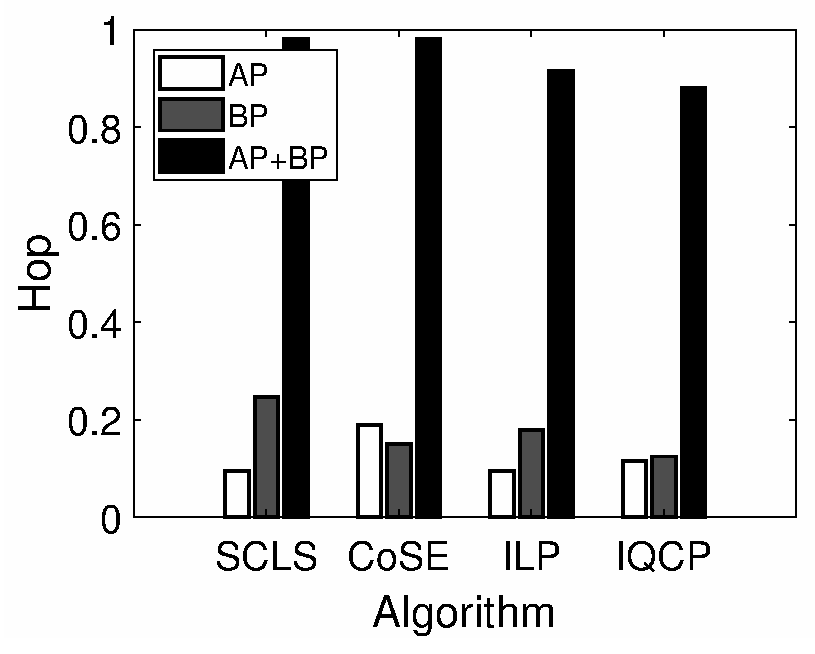
\includegraphics[width=2.25in]{figures/hop}
\caption{路径跳数}
\label{fig:normalization hop}
\end{minipage}
\end{figure}


\begin{figure*}[htbp]
\centering
\begin{minipage}[t]{0.3\linewidth}
\centering
\includegraphics[width=2.25in]{figures/runtime}
\caption{运行时间}
\label{fig:normalization runtime}
\end{minipage}
\hfill
\begin{minipage}[t]{0.3\linewidth}
\centering
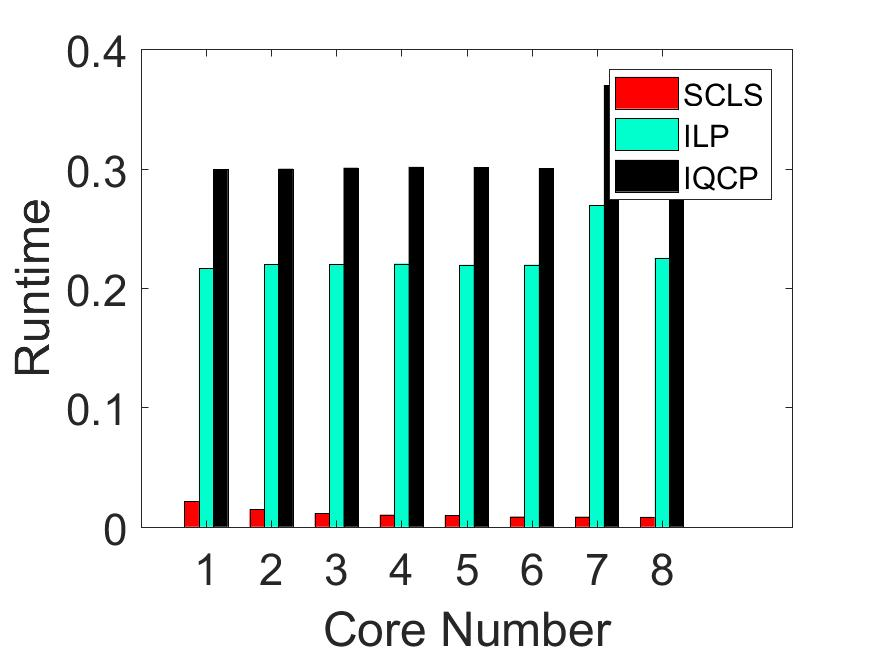
\includegraphics[width=2.25in]{figures/Runtime_noKSP_noCOSE}\\
  \caption{运行时间(无CoSE)}\label{fig:Runtime_noKSP_noCOSE}
\end{minipage}
\hfill
\begin{minipage}[t]{0.3\linewidth}
\centering
\includegraphics[width=2.25in]{figures/speedup}
\caption{核加速比}
\label{fig:Speedup}
\end{minipage}
\end{figure*}


\begin{figure*}[htbp]
\centering
\begin{minipage}[t]{0.3\linewidth}
\centering
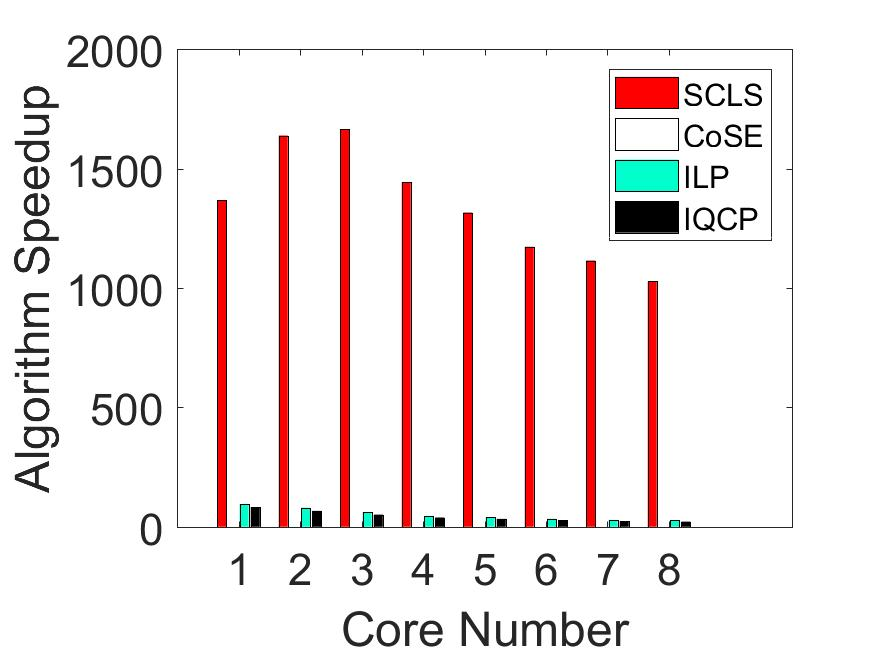
\includegraphics[width=2.25in]{figures/Multiple}
\caption{算法加速比}
\label{fig:Multiple}
\end{minipage}
\hfill
\begin{minipage}[t]{0.3\linewidth}
\centering
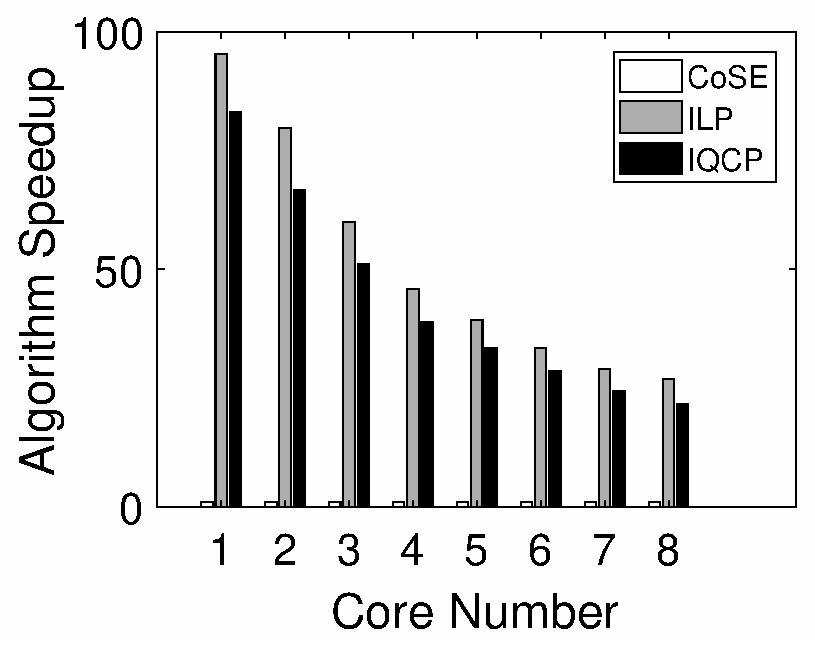
\includegraphics[width=2.25in]{figures/MultipleNoSCLS}
\caption{算法加速比(无SCLS)}
\label{fig:MultipleNoSCLS}
\end{minipage}
\hfill
\begin{minipage}[t]{0.3\linewidth}
\centering
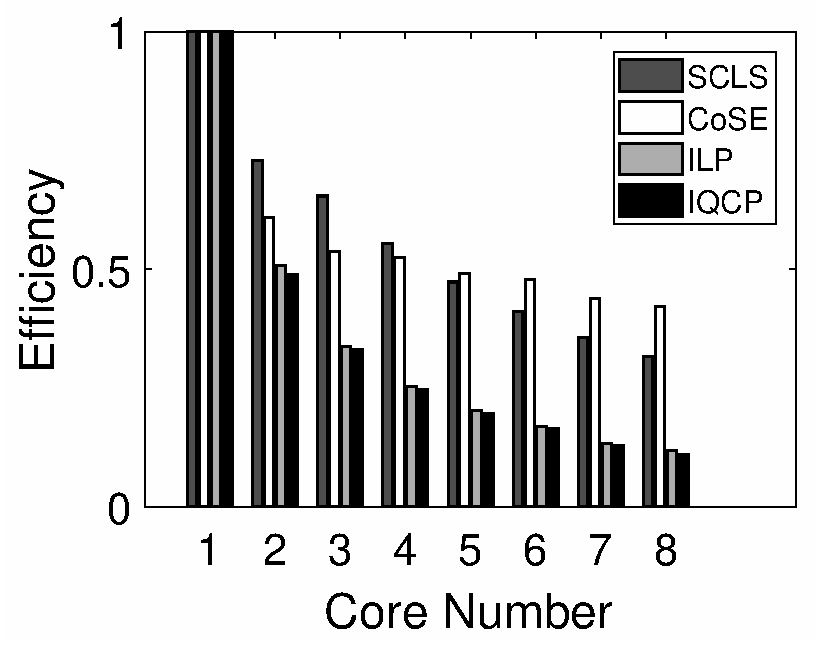
\includegraphics[width=2.25in]{figures/Efficiency}
 \caption{效率}
 \label{fig:Efficiency}
\end{minipage}
\end{figure*}
\section{小结}
本章提出了一种创新的分而治之算法,该算法能在遇到陷阱问题时将原有的min-min SRLG 不相交路由问题划分为多个并行执行子问题。与现有技术相比,这样的解决方案在搜索过程可以利用现有的AP 搜索结果,并且并行执行来加快路径查找。

